\subsection{Kernel density estimation : {\tt kernel\_density\index{kernel\_density}}, {\tt kde\index{kde}}}
{\tt kernel\_density} (alias : {\tt kde}) accepts a list of samples $L=[X_1,X_2,\dots,X_n]$ and optionally a sequence of options. It performs kernel density estimation\footnote{For the details on kernel density estimation and its implementation see~: Artur Gramacki, {\it Nonparametric Kernel Density Estimation and Its Computational Aspects}, Springer, 2018.} (KDE), optionally restricted to an interval $[a,b]$, to obtain an estimate $\hat{f}$ of the (unknown) probability density function $f$ from which the samples are drawn, defined by~:
\begin{equation}\label{eq:kde1}
  \hat{f}(x)=\frac{1}{n\,h}\,\sum_{i=1}^nK\left(\frac{x-X_i}{h}\right),
\end{equation}
where $K$ is the Gaussian kernel $K(u)=\frac{1}{\sqrt{2\,\pi}}\,\exp\left(-\frac{1}{2}\,u^2\right)$ and $h$ is the positive real parameter called the \emph{bandwidth}.

The supported options are listed below.
\begin{itemize}
  \item {\tt output=<type>} or {\tt Output=<type>} : specifies the form of the return value $\hat{f}$, where {\tt <type>} may be
  \begin{itemize}
    \item {\tt exact} : $\hat{f}$ is returned as the sum of Gaussian kernels, i.e.~as the right side of~\eqref{eq:kde1}, which is usable only when the number of samples is relatively small (up to few hundreds),
    \item {\tt piecewise} : $\hat{f}$ is returned as a piecewise expression obtained by the spline interpolation of the specified degree (by default, the interpolation is linear) on the interval $[a,b]$ segmented to the specified number of bins,
    \item {\tt list} (the default) : $\hat{f}$ is returned in discrete form, as a list of values $\hat{f}\left(a+k\,\frac{b-a}{M-1}\right)$ for $k=0,1,\dots,M$, where $M$ is the number of bins.
  \end{itemize}
  \item {\tt bandwidth=<value>} : specifies the bandwidth. {\tt <value>} may be
  \begin{itemize}
    \item a positive real number $h$,
    \item {\tt select} (the default) : bandwidth is selected using a direct plug-in method,
    \item {\tt gauss} or {\tt normal} or {\tt normald} : the Silverman's rule of thumb is used for selecting bandwidth (this method is fast but the results are close to optimal ones only when $f$ is approximately normal).
  \end{itemize}
  \item {\tt bins=<posint>} (by default 100) : the number of bins for simplifying the input data. Only the number if samples in each bin is stored. Bins represent the elements of an equidistant segmentation of the interval $S$ on which KDE is performed. This allows evaluating kernel summations using convolution when {\tt output} is set to {\tt piecewise} or {\tt list}, which significantly lowers the computational burden for large values of $n$ (say, few hundreds or more). If {\tt output} is set to {\tt exact}, this option is ignored.
  \item {\tt [range=]a..b} or {\tt range=[a,b]} or {\tt x=a..b} : the interval $[a,b]$ on which KDE is performed. If an identifier $x$ is specified, it is used as the variable of the output. If the range endpoints are not specified, they are set to $a=\min_{1\leq i\leq n} X_i-3\,h$ and $b=\max_{1\leq i\leq n}X_i+3\,h$ (unless {\tt output} is set to {\tt exact}, in which case this option is ignored).
  \item {\tt interp=<posint>} (by default 1) : the degree of the spline interpolation, ignored unless {\tt output} is set to {\tt piecewise}.
  \item {\tt spline=<posint>} : sets {\tt option} to {\tt piecewise} and {\tt interp} to {\tt <posint>}.
  \item {\tt eval=x0} : only the value $\hat{f}(x_0)$ is returned (this cannot be used with {\tt output} set to {\tt list}).
  \item an unassigned identifier {\tt x} (by default $x$) : the variable of the output.
  \item {\tt exact} : the same as {\tt output=exact}.
  \item {\tt piecewise} : the same as {\tt output=piecewise}.
\end{itemize}

\paragraph{Examples.}
Input :
\begin{center}
  \tt kernel\_density([1,2,3,2],bandwidth=1/4,exact)
\end{center}
Output :
\begin{center}
  \tt 0.4*(exp(-8*(x-3)\verb|^|2)+2*exp(-8*(x-2)\verb|^|2)+exp(-8*(x-1)\verb|^|2))
\end{center}
Input :
\begin{center}
  \tt f:=unapply(normald(4,1,x)/2+normald(7,1/2,x)/2,x); plot(f(x),x=0..10)
\end{center}
Output :
\begin{center}
  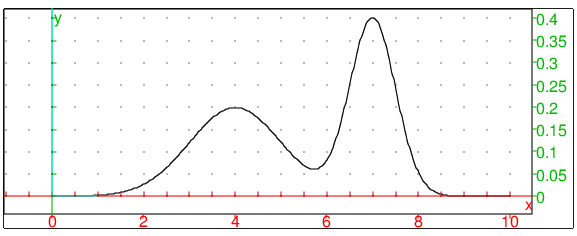
\includegraphics[width=0.75\textwidth]{kde_plot1.png}
\end{center}
Input :
\begin{center}
  \tt X:=randvar(f,range=0..10,1000):; S:=sample(X,1000):; F:=kernel\_density(S,piecewise):; plot([F,f(x)],x=0..10, display=[line\_width\_2+blue,line\_width\_1+black])
\end{center}
Output :
\begin{center}
  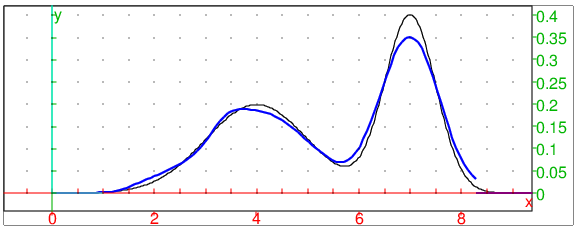
\includegraphics[width=0.75\textwidth]{kde_plot2.png}
\end{center}
Input :
\begin{center}
  \tt kernel\_density(S,bins=50,spline=3,eval=4.75)
\end{center}
Output :
\begin{center}
  \tt 0.14655478136
\end{center}
Input :
\begin{center}
  \tt time(kernel\_density(sample(X,1e5),piecewise))
\end{center}
Output :
\begin{center}
  \tt "Done",[0.17,0.1653323]
\end{center}
Input :
\begin{center}
  \tt S:=sample(X,5000):; sqrt(int((f(x)-kde(S,piecewise))\verb|^|,x=0..10))
\end{center}
Output :
\begin{center}
  \tt 0.0269841239243
\end{center}
Input :
\begin{center}
  \tt S:=sample(X,25000):; sqrt(int((f(x)-kde(S,bins=150,piecewise))\verb|^|2,x=0..10))
\end{center}
Output :
\begin{center}
  \tt 0.0144212781377
\end{center}
